\documentclass[letterpaper]{article}

\usepackage{natbib,alifeconf}  %% The order is important
\usepackage{graphicx}%
\usepackage{blindtext}
\usepackage{subfig}


% *****************
%  Requirements:
% *****************
%
% - All pages sized consistently at 8.5 x 11 inches (US letter size).
% - PDF length <= 8 pages for full papers, <=2 pages for extended
%    abstracts (not including citations).
% - Abstract length <= 250 words.
% - No visible crop marks.
% - Images at no greater than 300 dpi, scaled at 100%.
% - Embedded open type fonts only.
% - All layers flattened.
% - No attachments.
% - All desired links active in the files.

% Note that the PDF file must not exceed 5 MB if it is to be indexed
% by Google Scholar. Additional information about Google Scholar
% can be found here:
% http://www.google.com/intl/en/scholar/inclusion.html.


% If your system does not generate letter format documents by default,
% you can use the following workflow:
% latex example
% bibtex example
% latex example ; latex example
% dvips -o example.ps -t letterSize example.dvi
% ps2pdf example.ps example.pdf


% For pdflatex users:
% The alifeconf style file loads the "graphicx" package, and
% this may lead some users of pdflatex to experience problems.
% These can be fixed by editing the alifeconf.sty file to specify:
% \usepackage[pdftex]{graphicx}
%   instead of
% \usepackage{graphicx}.
% The PDF output generated by pdflatex should match the required
% specifications and obviously the dvips and ps2pdf steps become
% unnecessary.


% Note:  Some laser printers have a serious problem printing TeX
% output. The use of ps type I fonts should avoid this problem.


\title{Towards Ecosystem Management from Greedy Reinforcement Learning in a Predator-Prey Setting}
\title{Emergent Cooperation from Greedy Multi-Agent Reinforcement Learning in a Predator-Prey Setting}
\author{Fabian Ritz Ratke$^{1}$, Daniel Ratke$^{1}$, Thomy Phan$^1$ \and Claudia Linnhoff-Popien$^1$ \\
\mbox{}\\
$^1$Mobile and Distributed Systems Group, LMU Munich, Germany \\
$^2$LMU Munich, Germany \\
D.Ratke@campus.lmu.de} % email of corresponding author

% For several authors from the same institution use the same number to
% refer to one address.
%
% If the names do not fit well on one line use
%         Author 1, Author 2 ... \\ {\Large\bf Author n} ...\\ ...
%
% If the title and author information do not fit in the area
% allocated, place \setlength\titlebox{<new height>} after the
% \documentclass line where <new height> is 2.25in



\begin{document}
\maketitle

\begin{abstract}
% Abstract length should not exceed 250 words
    \blindtext[2]
\end{abstract}

\section{Introduction}

\blindtext[4]

\begin{figure}%
    \centering
    \subfloat[][\centering Two predators and multiple prey]{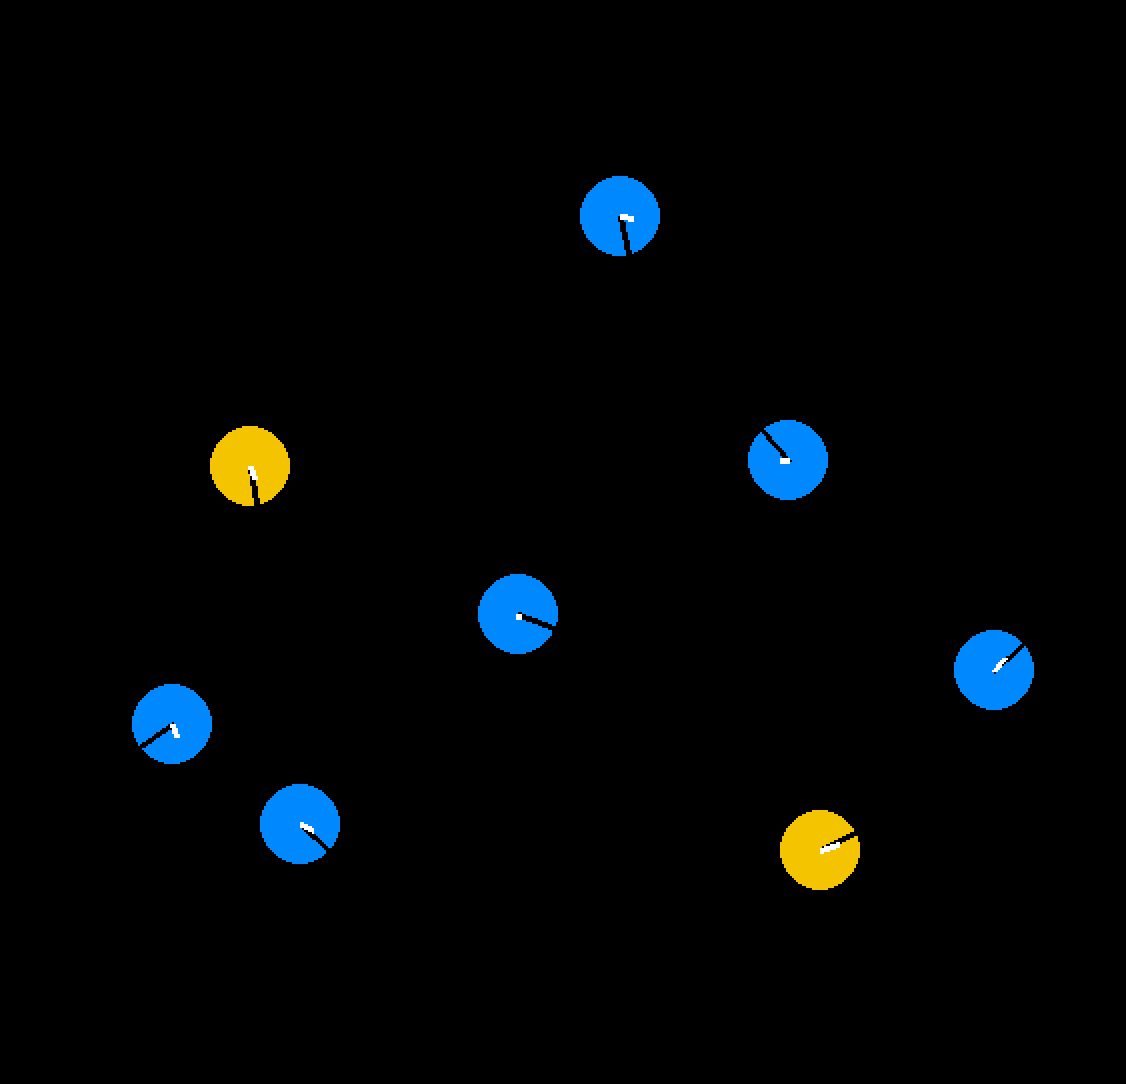
\includegraphics[width=3.8cm]{figures/game_screen2.png} }%
    \subfloat[][\centering A stunned predator]{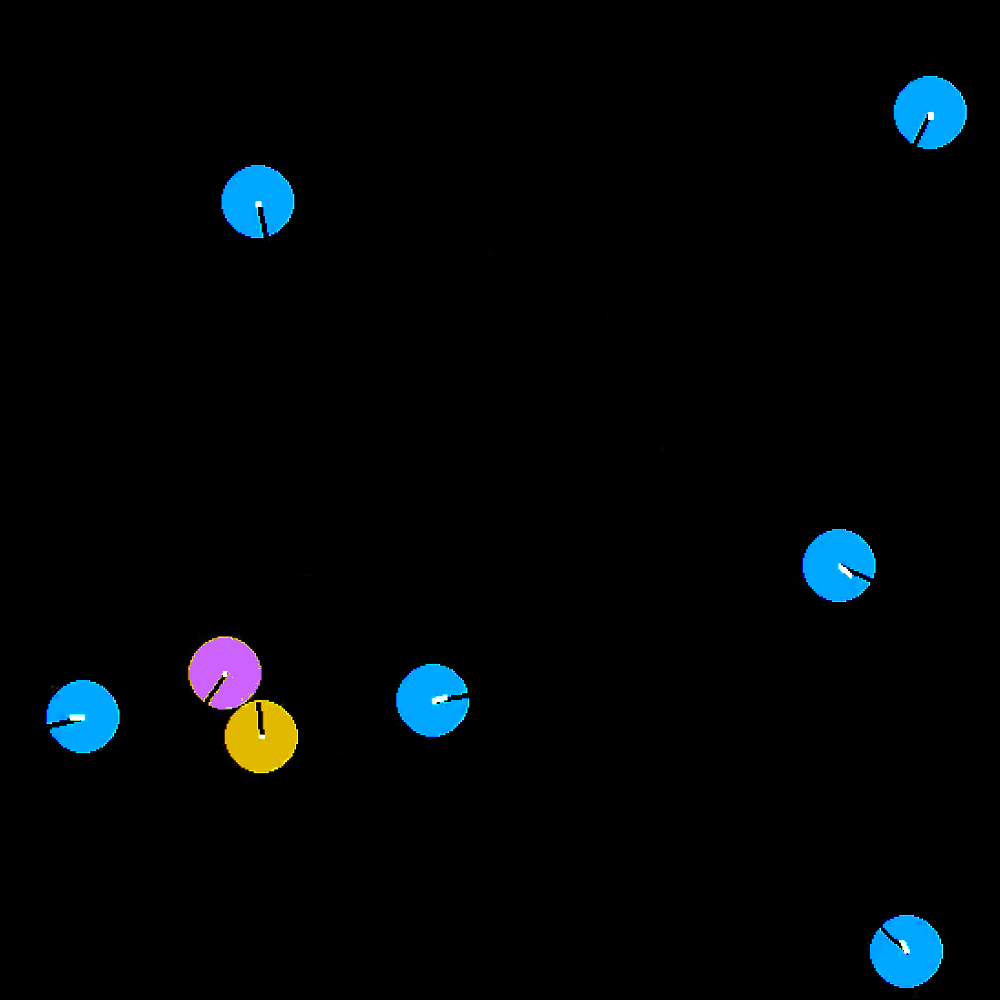
\includegraphics[width=3.66cm]{figures/stun_move2.png} }%
    \caption{The predator-prey environment, with yellow predators and blue prey. Predators can stun each other --- a stunned predator appears purple and cannot move for a certain number of steps.}%
    \label{fig:aquarium}%
\end{figure}

\section{Background}

\subsection{Reinforcement Learning}

\blindtext[2]

\subsection{Multi-Agent Reinforcement Learning}

\blindtext[3]

\subsection{Herding Behaviour}

\blindtext[2]

\subsection{Cooperation}

\blindtext[2]

\subsection{Related Work}

\blindtext[5]

\section{Aquarium Environment}

\blindtext[5]

\section{Experimental Setup}

\blindtext[2]

\section{Results}

TODO: Define sustainability

\begin{figure*}%
    \centering
    \subfloat[][\centering Sustainability with 1 initial fish.]{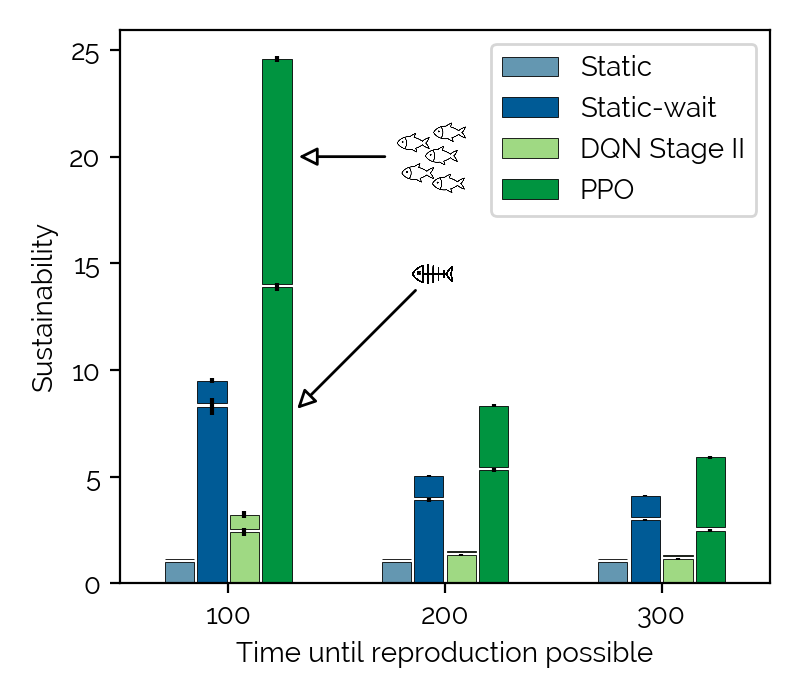
\includegraphics[width=7.5cm]{figures/dqncomp1fish_2.png} }%
    \subfloat[][\centering Sustainability with 2 initial fishes.]{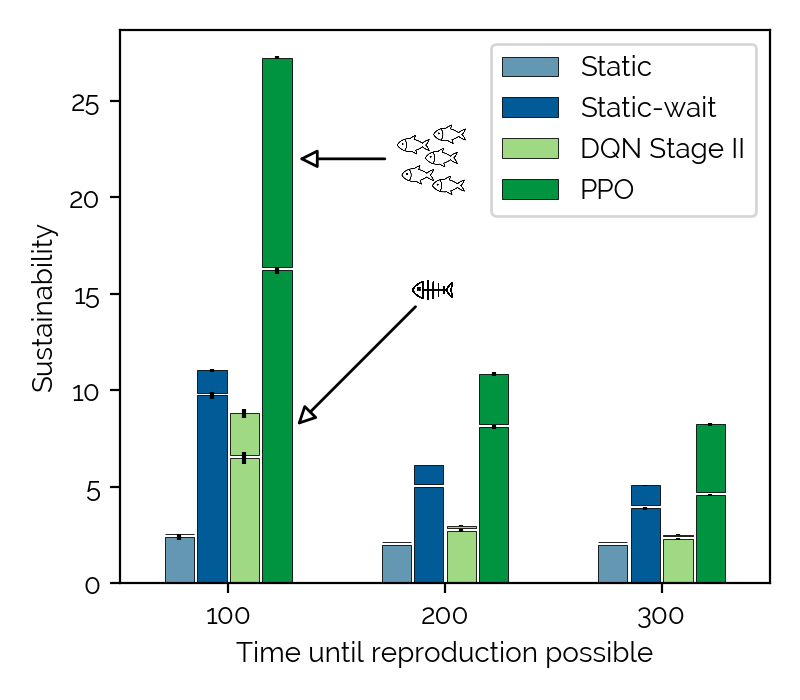
\includegraphics[width=7.5cm]{figures/dqncomp2fish_2.png} }%
    \caption{Sustainability of static, static-wait, DQN Stage II and PPO. PPO consistently leads to the most sustainable behavior due to herding a rather large fish population, which results in a higher rate of fish procreations and thus more prey to be caught. 20 models were trained for each DQN Stage II and PPO for each scenario.}
    \label{fig:dqncomp}%
\end{figure*}

\begin{figure}[t]
\begin{center}
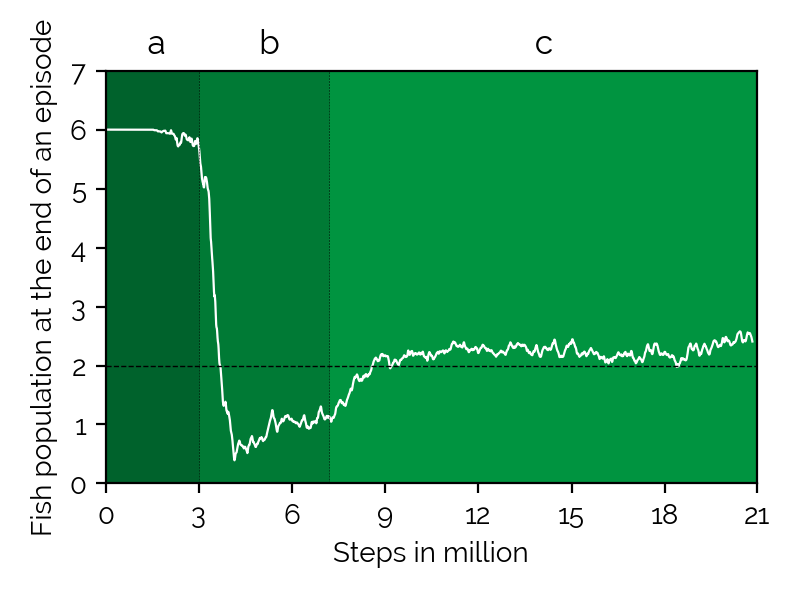
\includegraphics[width=8cm]{figures/fish_pop_chart3.png}
    \caption{Left-over fish population per learning episode over 12M steps. In this setting there is at maximum 6 fishes in the population. When sharks learn to herd fishes, they go through 3 stages. Stage $a$, in which they cannot hunt effectively yet and thus leave the full population intact at the end of the episode. Stage $b$, in which they effectively hunt and overhunt, leaving no fishes at the end of the epsiode. Lastly, stage $c$, in which they learn to keep a herd of 2 fishes around, up until the end of the epsiode.}
\label{fig:fish_pop}
\end{center}
\end{figure}

\begin{figure}[t]
\begin{center}
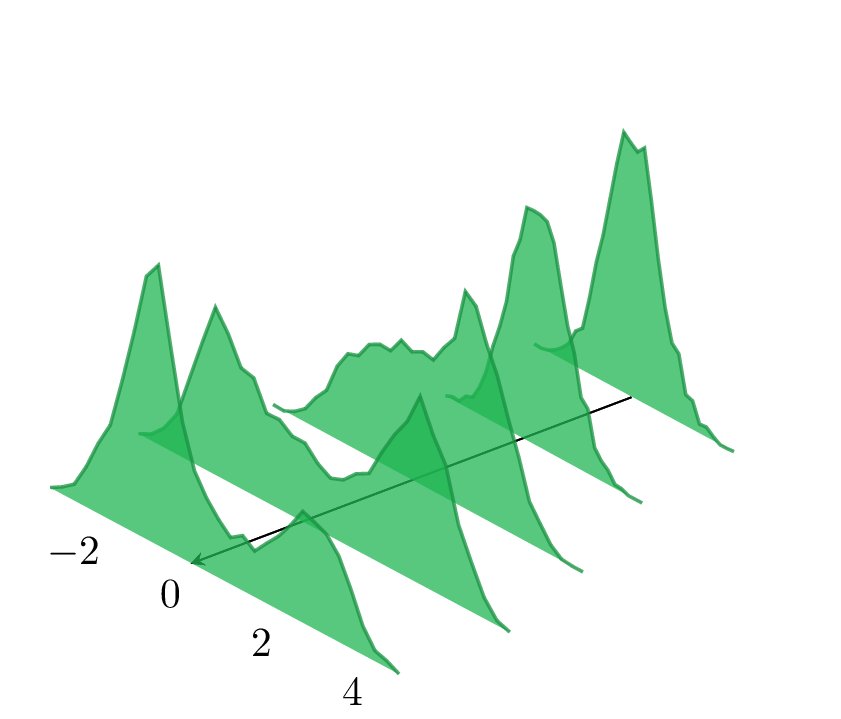
\includegraphics[width=6cm]{figures/shark_speeds.png}
\caption{From back to front: Distribution of shark speeds over time. When sharks learn to herd fishes, the distribution of their speed becomes bimodal after a while --- suggesting that sometimes they wait while other times they actively hunt at high speed.}
\label{fig:shark_speeds}
\end{center}
\end{figure}

TODO: Define active herding.

\begin{figure*}[t]
\begin{center}
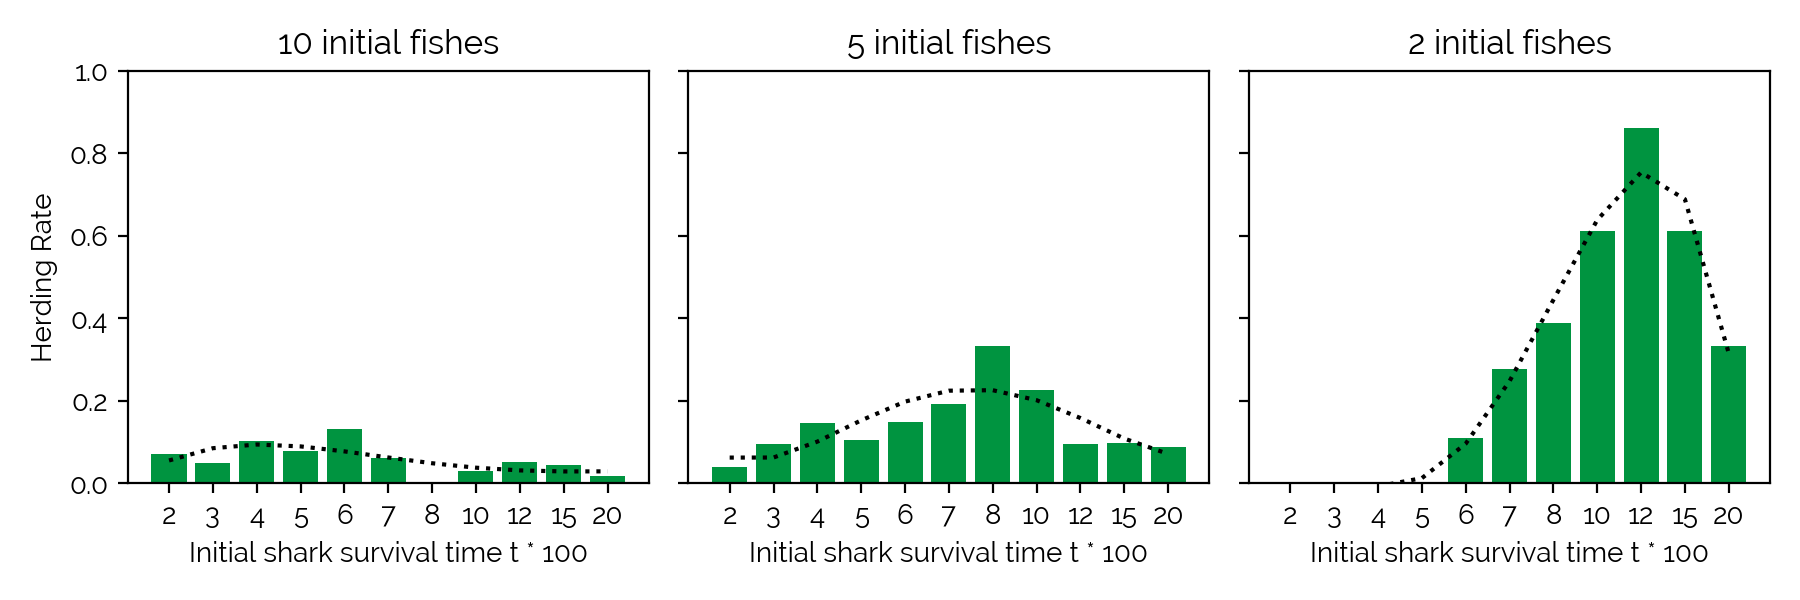
\includegraphics[width=.9\textwidth]{figures/herding.png}
    \caption{Herding rate in different scenarios. From left to right, initial fish population is decreased (10, 5, 2). A lower fish population increases sustainability pressure --- the sharks get into the situation of 0 left fishes much quicker. Further, each scenario varies the initial shark survival time. Especially in the scenario with just two fishes the importance of this parameter becomes clear --- giving the sharks an initial 1200 steps induces the highest rate of herding. While low initial survival steps induce too much survival pressure, thus overriding any sustainability with the need for survival, too high initial survival steps do not induce enough pressure, reducing the need for active herding as the sharks now often do not actively hunt but just idle. The curve was fitted using 4 polynomials and each bar represents 20 models.}
\label{fig:herding}
\end{center}
\end{figure*}

\begin{figure*}[t]
\begin{center}
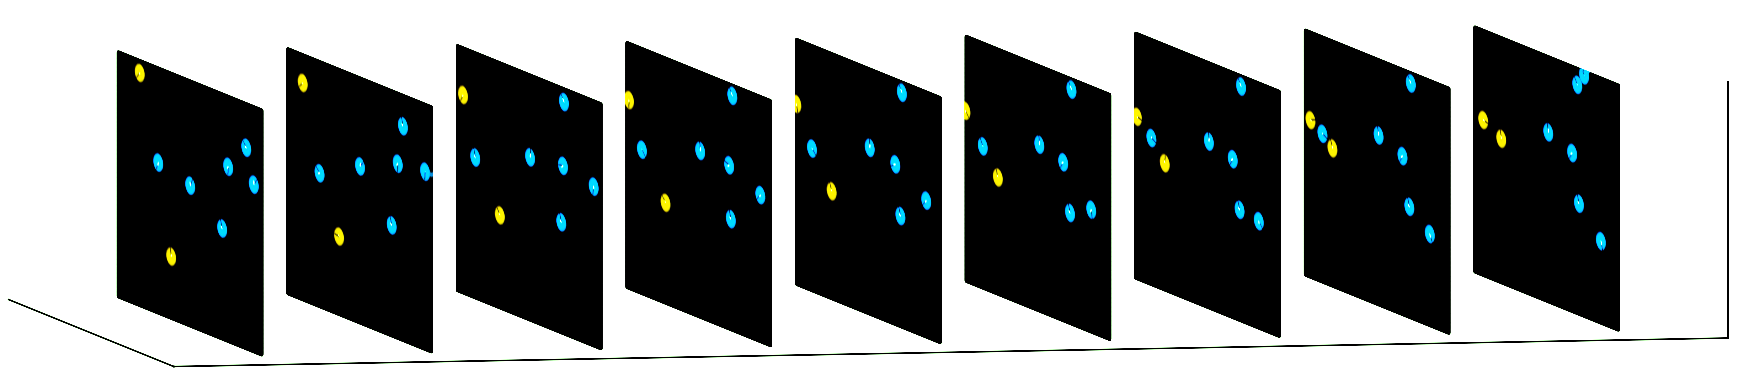
\includegraphics[width=.9\textwidth]{figures/coop_movie_frames2.png}
\caption{From left to right: Two sharks cooperatively catch a fish.}
\label{fig:coop_movie}
\end{center}
\end{figure*}

\begin{figure*}%
    \centering
    \subfloat[][\centering Cooperation rate with initial fish population of 10.]{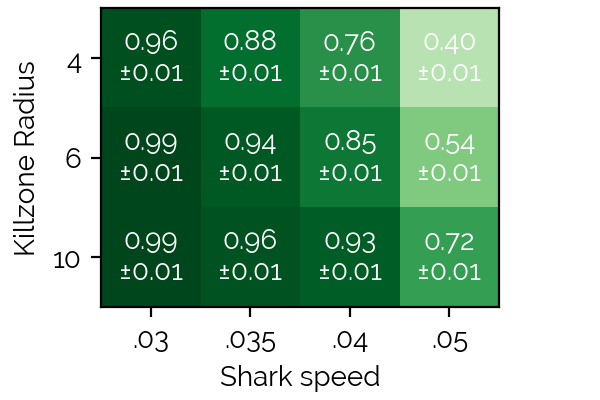
\includegraphics[width=5.5cm]{figures/coop_chart_split1.png} }%
    \subfloat[][\centering Cooperation rate with initial fish population of 5.]{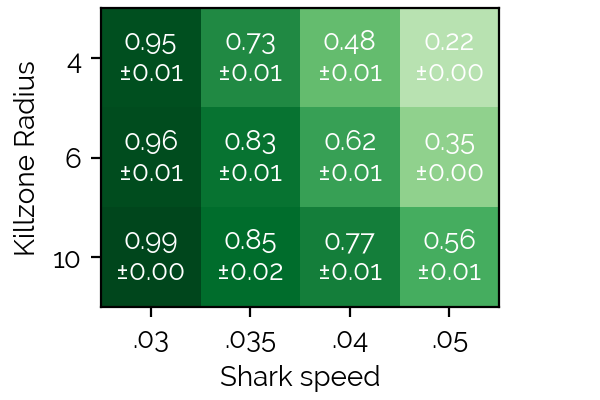
\includegraphics[width=5.5cm]{figures/coop_chart_split2.png} }%
    \subfloat[][\centering Cooperation rate with initial fish population of 5 and stuns.]{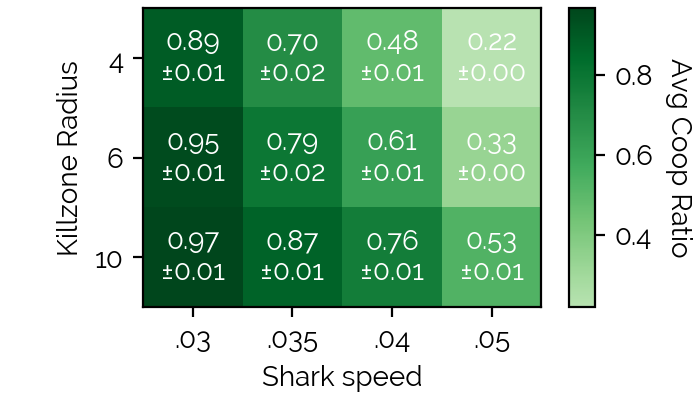
\includegraphics[width=6.5cm]{figures/coop_chart_stuns_split2.png} }%
    \caption{Cooperation rate in different scenarios. TODO: Analysis}%
    \label{fig:coop}%
\end{figure*}

\begin{figure*}[t]
\begin{center}
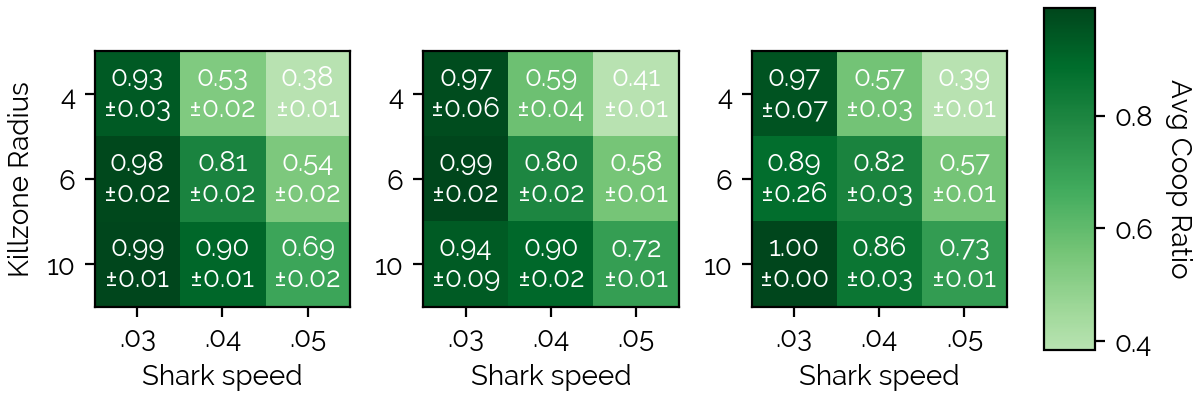
\includegraphics[width=14cm]{figures/coop_vs_sterberisiko_5fish.png}
\caption{Cooperation rate vs starving pressure with initial fish population of 5. TODO: Analysis}
\label{fig:coop_starve}
\end{center}
\end{figure*}

\blindtext[14]

\section{Conclusion}

\blindtext[2]

\footnotesize
\bibliographystyle{apalike}
\bibliography{paper} % replace by the name of your .bib file

\end{document}
